\documentclass{mise_en_page}

\usepackage{booktabs} % Required for the \toprule, \midrule and \bottomrule lines
\usepackage{array}
\usepackage{float}

\projet{Projet Ingéniérie}
\equipe{H4314}
\responsable{Tristan Delizy}
\redacteurs{Arnaud Lahache} % Optionnel
\titre{Dossier de Synthèse du projet COPEVUE-MONIT}
\version{1.3}
\objet{Ce dossier présentera la solution générale proposée par notre équipe dans le cadre du projet COPEVUE-MONIT}
\etat{validé} %draft, non relu, non validé, validé

\begin{document}

\maketitle

\begin{historique}
    \histo{1.0}{30/01/2012}{Initialisation du document}
    \histo{1.1}{06/02/2012}{Élaboration du contenu}
    \histo{1.2}{09/02/2012}{Finalisation du contenu}
    \histo{1.3}{12/02/2012}{Validation}
\end{historique}

\newpage

\tableofcontents

\section{Introduction}

\subsection{Objectif de ce dossier}
Le dossier de synthèse du projet COPEVUE-MONIT a pour objectif de présenter les principaux choix et les différentes élaborations de la solution proposée. Ce dossier aura pour but de présenter les nombreuses améliorations que notre solution pourrait impacter sur le système de la COPEVUE.

\section{Documents applicables et de référence}

\subsection{Documents de référence}

\begin{description}
	\item[QL / PAQP / PAQP] Plan d'assurance qualité du projet COPEVUE-MONIT, présentant notre démarche qualité au niveau \emph{projet}.
	\item[GLOSSAIRE / GL / glossaire ] Glossaire spécifique à la démarche qualité du projet.
\end{description}

\subsection{Documents applicables}

\begin{description}
	\item[AE / Etude de faisabilité] Dossier n°1 du projet COPEVUE-MONIT Présentant l'étude de faisabilité du projet.
	\item[ABTNS / STB ] Dossier n°2 du projet COPEVUE MONIT présentant la spécification technique des besoins du nouveau système.
	\item[DNS / Dossier de conception ] Dossier n°3 du projet COPEVUE-MONIT présentant la conception générale dans le cadre de la définition du nouveau système proposé.
\end{description}

\section{Terminologie et glossaire}

Les terminologies utilisées dans ce dossier sont spécifiques au projet COPEVUE-MONIT :

\begin{description}
	\item[GLOSSAIRE / GL / glossaire ] Glossaire commun à l'ensemble du projet COPEVUE-MONIT.
\end{description}

Vous pouvez donc vous référer à l'ensemble de ces documents pour tous les points concernants les terminaisons ainsi que le glossaire.

\section{Présentation de la solution proposée}

\subsection{Architecture}

\subsubsection{Architecture applicative}

\begin{figure}[H]
	\centering
	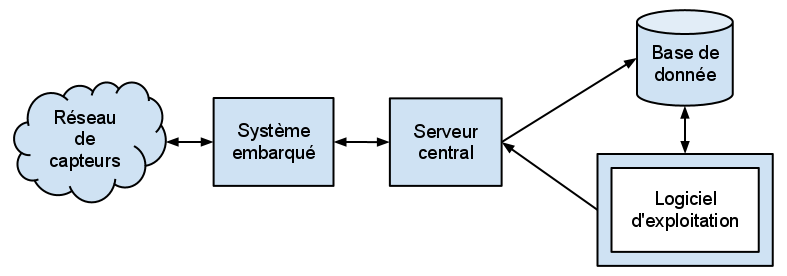
\includegraphics[width=150mm]{archi_app.png}
	\caption{Architecture applicative générale}
\end{figure}

\begin{figure}[H]
	\centering
	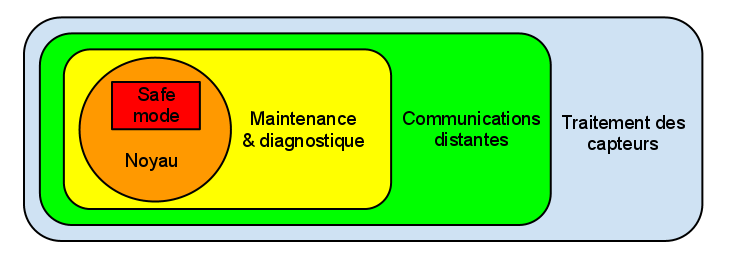
\includegraphics[width=150mm]{archi_embarque.png}
	\caption{Architecture applicative du système embarqué}
\end{figure}

\begin{figure}[H]
	\centering
	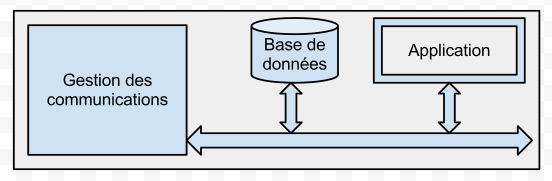
\includegraphics[width=150mm]{archi_serveur.png}
	\caption{Architecture applicative du serveur central}
\end{figure}

\subsubsection{Architecture technique}

\begin{figure}[H]
	\centering
	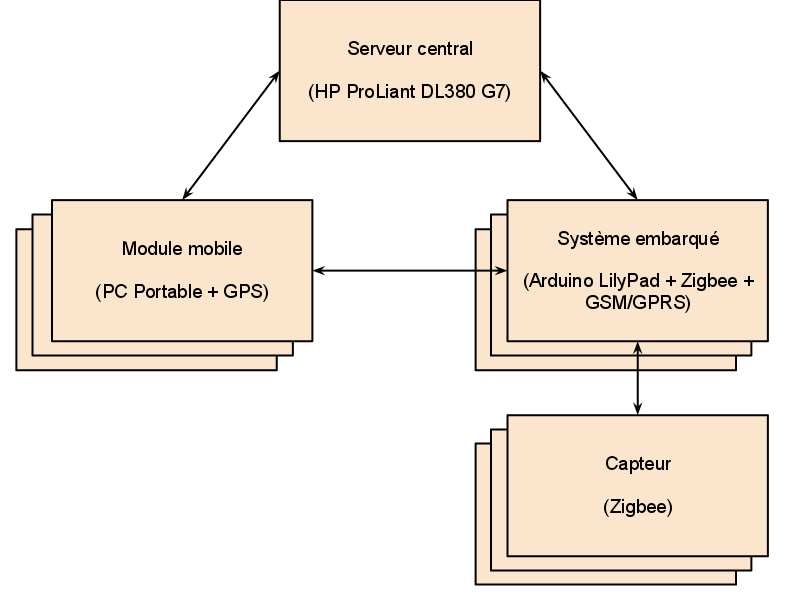
\includegraphics[width=150mm]{archi_tech.png}
	\caption{Architecture technique générale}
\end{figure}

\subsection{Fonctionement général}

\subsubsection{Site isolé}

\begin{figure}[H]
	\centering
	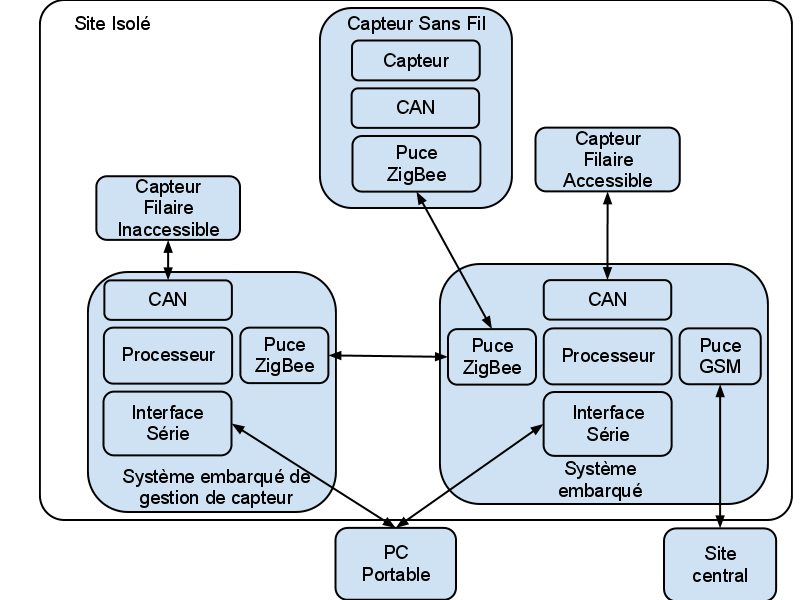
\includegraphics[width=150mm]{site_isole.png}
	\caption{Architecture détaillée d'un site isolé}
\end{figure}

Le système embarqué décrit dans la figure çi-dessus comportera :

\begin{itemize}
	\item Comme processeur une carte Arduino LilyPad
	\item Un module de communication ZigBee ou XBee
	\item Une puce GSM/GPRS Quectel M10
\end{itemize}

\begin{figure}[H]
	\centering
	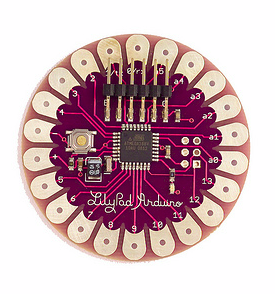
\includegraphics[width=50mm]{arduino.png}
	\caption{Carte basse consommation Arduino LilyPad}
\end{figure}

\begin{figure}[H]
	\centering
	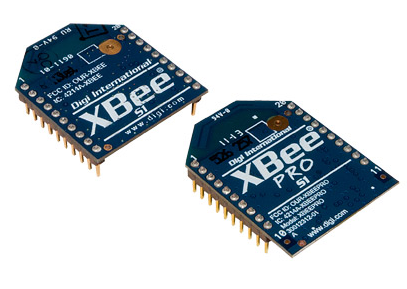
\includegraphics[width=50mm]{zigbee.png}
	\caption{Module ZigBee/XBee PRO}
\end{figure}

\subsubsection{Site central}

\begin{figure}[H]
	\centering
	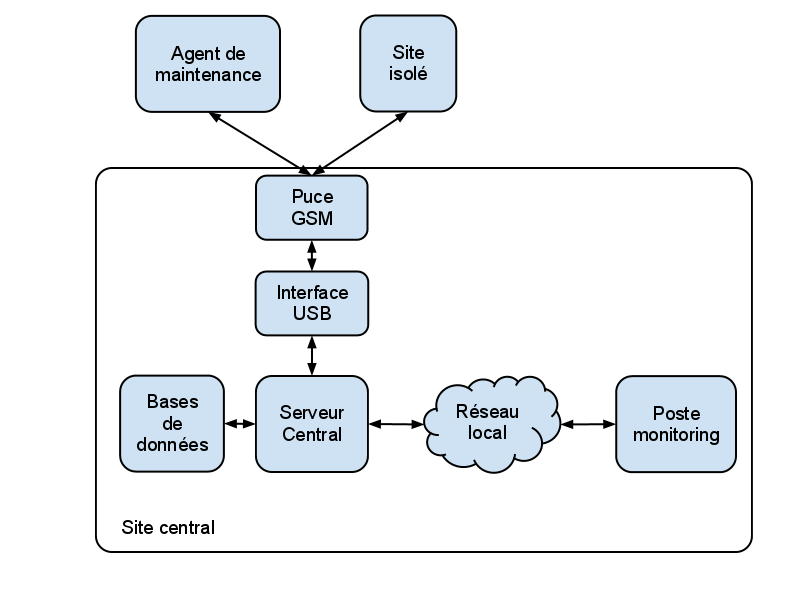
\includegraphics[width=150mm]{site_central.png}
	\caption{Architecture détaillée du site central}
\end{figure}

\subsubsection{Apports énergétique}

La solution énergétique que nous proposons est l'utilisation d'accumulateurs longue durée (Ni/Zn) remplaçables durant les opérations de maintenance (par des batteries équivalentes déjà chargées)

\begin{description}
	\item[Apport en station filaire]
		Utilisation d'une batterie centralisée qui alimente à fois les capteurs et le système embarqué
	\item[Apport en station non filaire]
		Utilisation de piles pour chaque capteur, le système embarqué étant alimenté par sa propre batterie
	\item[Apport en station hybride]
		Utilisation de batterie centralisée pour alimenter le système embarqué et les capteurs proches qui sont reliés. Les autres capteurs sont alimentés par piles.
\end{description}

\begin{figure}[H]
	\centering
	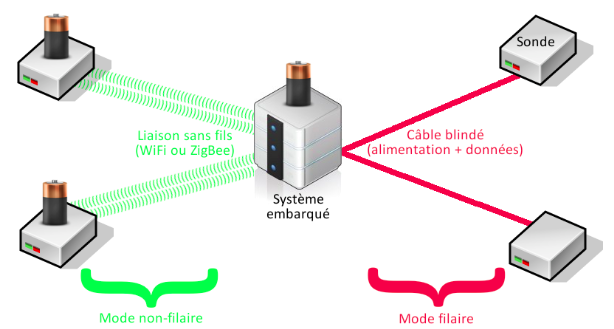
\includegraphics[width=150mm]{hybride.png}
	\caption{Architecture d'un site hybride}
\end{figure}

\subsubsection{Communication}

\begin{figure}[H]
	\centering
	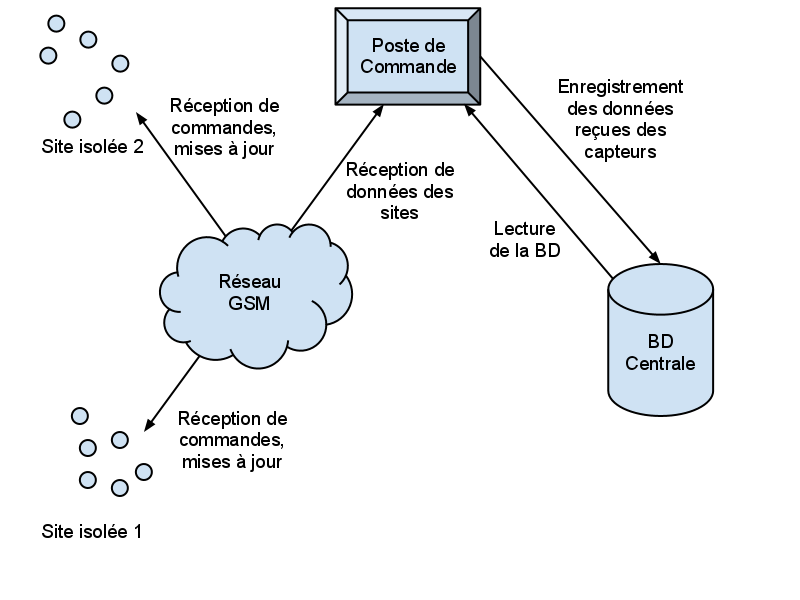
\includegraphics[width=150mm]{donnees.png}
	\caption{Communications de données}
\end{figure}

\subsubsection{Données}

\begin{figure}[H]
	\centering
	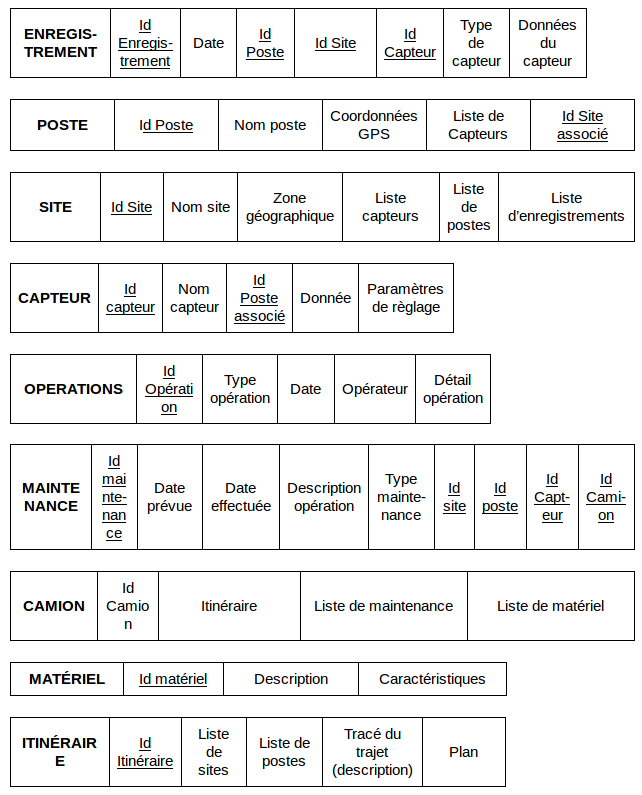
\includegraphics[width=150mm]{tables.png}
	\caption{Modélisation des données}
\end{figure}

\subsection{Apports de la solution proposée}

\subsubsection{Thèmes de progrès}

Notre système doit améliorer certains points qui ne sont pour le moment pas encore mis en place sur les sites. Il doit permettre une diminution des coûts de trajet, réduire l’impact écologique des trajets des opérations de livraison et de maintenance par la mise en place d’un système d’aide à la décision et de gestion de trajets optimaux. Ceci devra également être géré par la gestion de tous les sites en temps réel basée sur un traitement en continu des données en provenance des sites. Ce suivi pourra aboutir à une traçabilité des opérations et de l’état des sites par l’utilisation de bases de données stockées sur serveurs qui pourront gérer des règles d’anticipation des opérations de maintenance et de livraison à réaliser. Ces règles pourront être traitées, configurées voire générées par l’utilisation d’un module d’intelligence artificielle axé sur l’aide à la décision.

Les différents axes de progrès retenus sont les suivants :

\begin{description}
	\item[Réduire les déplacements humains coûteux et polluants]
		Notre système doit être capable de traiter les données récupérées des différents sites de manière à déterminer des solutions optimisées pour plusieurs critères.
	\item[Suivi temps réel]
		La mise en place de notre système permettra un suivi constant en temps réel de tous les sites isolés, peu importe leur position et les difficultés rencontrées pour y accéder
	\item[Traçabilité des opérations et de l’état du système]
		La mise en place d’un central chargé de collecter toutes les données en temps réel permet à la fois d’établir un historique des différents relevés, mais aussi de prévoir les opérations de maintenance à effectuer. Toutes ces données informatiques peuvent en effet être traitées intelligemment afin de mettre en place un suivi à long terme de chacun des sites
\end{description}

\subsubsection{Coûts de la solution}

Notre solution emploiera de nombreux équipements qu’il nous faudra nous procurer. Certains d’entre-eux sont relativement très coûteux notamment pour assurer une bonne sécurité ou pour avoir une bonne précision des mesures.

\section{Mise en place du système}

\subsubsection{Mise en place de l'architecture technique et applicative}

\begin{description}
	\item[Architecture technique]
		La mise en place de l'architecture technique dépendra du type de site : en effet, nous proposons 3 configurations différentes (filaire, non filaire, hybride). De plus, les conditions extrêmes de certains sites peuvent amener quelques changements. Heureusement, le matériel utilisé est suffisament résistant.
	\item[Architecture applicative]
		La mise en place de l'architecture applicative ne posera pas de problème pour les systèmes embarqué (les cartes contiendront directement l'application), mais les autres applications comme celle du monitoring nécessiteront une installation ainsi qu'une configuration afin de s'adapter à votre système.
\end{description}

\subsubsection{Intégration avec le système existant}

La solution proposée a été rédigée en respectant le désir de la COPEVUE de vouloir l'intégrer avec le système existant. Ainsi l'ensemble des composants utilisés peuvent tout à fait réutiliser les composants des sites existants.

\end{document}
